\documentclass[12pt,a4paper,twoside]{report}
\usepackage[pdfborder={0 0 0}]{hyperref}
\usepackage[margin=25mm]{geometry}
\usepackage{graphicx}
\usepackage{parskip}
\usepackage{enumerate}
\usepackage[utf8]{inputenc}
\usepackage{amsmath}
\usepackage{amsfonts}
\usepackage{float}
\graphicspath{ {Images/} }



% For temporarily splitting the document into multiple columns
\usepackage{multicol}

% Command for extracting the word count.
\newcommand\wordcount{\input{word.count}}

\begin{document}

% Title Page
\begin{titlepage}
	\noindent
	\begin{minipage}[t][][t]{0.5\textwidth}
		
\includegraphics[width=40mm]{CamLogo.jpg}
	\end{minipage}
	\begin{minipage}{0.5\textwidth}
	\begin{flushright}
		\large
		\textit{Harry Graham}
		\\
		\textit{Christ's College}
		\\
		\texttt{hg402}
	\end{flushright}
	\end{minipage}
	
	\begin{center}
	\vspace{6cm}
	{\sc\large Computer Science Tripos - Part II Project\par}
	\vspace{0.5cm}
	{\huge\bf Deep Learning Techniques for Credit Card Fraud Detection\par}
	\vspace{0.5cm}
	{\large May 18, 2018 \par}
	\end{center}

\end{titlepage}

\pagestyle{plain}

\section*{\huge Proforma}
\vspace{0.5cm}
{\large
\begin{tabular}{ll}
Name:               & \bf Harry Graham \\
College:            & \bf Christ's College \\
Project Title:      & \bf Deep Learning Techniques for Credit Card Fraud \\
			 & \bf Detection \\
Examination:        & \bf Computer Science Tripos -- Part II, June 2018 \\
Word Count:         &  \\
Project Originators: & H.~Graham \& B.~Dimanov \\
Supervisors:         & Dr M.~Jamnik \& B.~Dimanov 
\end{tabular}
}

\section*{Original Aims of the Project}
The primary aim of the project was to implement and compare some deep learning techniques, alongside some baseline models, for credit card fraud detection (CCFD). More specifically, I aimed to experiment with two popular types of architecture, namely Convolutional Neural Networks (CNNs)  \cite{DBLP:journals/corr/SimonyanZ14a} and Generative Adversarial Networks (GANs). These have been successful in the image classification space and the aim of this project was to shed light on their use in the credit card fraud space. This kind of experimentation of predominantly image-based models, on single dimensional, time-series data is a relatively novel approach for CCFD.

\section*{Work Completed}
All of the core project aims set out in the proposal have been met, meaning results have been collated and evaluated across the three main components of the project: Baseline Models, CNN methods and GAN methods. 
I have also gone on to do some extension work relating to further investigation on the models I have experimented with. This is in the form of parameter tuning and further analysis not originally set out in the project proposal.

\section*{Special Difficulties}
None.


\newpage
\section*{Declaration}

I, Harry Graham of Christ's College, being a candidate for Part II of the Computer Science Tripos, hereby declare that this dissertation and the work described in it are my own work, unaided except as may be specified below, and that the dissertation does not contain material that has already been used to any substantial extent for a comparable purpose.

\vspace{1cm}
\begin{multicols}{2}

\rule{5cm}{0.15mm} \\
\leftline{\scshape{Signed}}

\columnbreak

\rule{5cm}{0.15mm} \\
\leftline{\scshape{Date}}

\end{multicols}


\tableofcontents

\pagestyle{headings} 

\chapter{Introduction}

Credit card fraud is a globally significant and increasing problem. According to the Nilson Report \cite{nilsonreport}, annual global fraud losses reached \$22.80 billion in 2016, up 4.4\% over 2015. Machine learning has contributed a lot to this problem over the years, helping to automatically learn to classify fraudulent transactions. However, this is still somewhat tedious and clearly, the money lost due to fraud is not decreasing. Not to mention, we still have this difficult business decision of when to draw the cutoff points between classifying fraud but perhaps allowing more benign transactions to be blocked.

A lot of machine learning concepts have been around for decades but ongoing research into deep learning architectures and their applications, makes for an interesting experimentation space. In this project I explore the performance of some particular models, focusing on deep learning, applied to the particular problem of credit card fraud detection (CCFD).

In particular, the aim is to shed light on the use of architectures that have had success in the image classification/generation space, in the context of non-image data i.e transactional vectors and time series data.
This is something that has recently seen some success \cite{wang2017time} and is novel to credit card fraud data. 
I first explore a set of baseline classifiers, which are primarily a handful of out-of-the-box supervised learning classifiers such as Random Forest. The point of these is to set the scene for experimenting with the data and to see what can be achieved with what is easily available, in other words without any 'deep' learning components. Here, I also establish techniques and methods for processing and evaluating the data i.e cross-validation, datapoint scaling, and data visualisation. 

Then the project shifts to experimenting with Convolutional Neural Networks (CNNs) \cite{DBLP:journals/corr/SimonyanZ14a} and Generative Adversarial Networks (GANs) \cite{2014arXiv1406.2661G}.  

\chapter{Preparation} \label{preparation}


\section{Convolutional Neural Networks}
\section{Generative Adversarial Networks}
GAN is a framework proposed by Ian Goodfellow, Yoshua Bengio and others in 2014. The idea is that we have two networks: a generator and a discriminator. The generator network tries to produce,  from random noise,  data in the form of the training data we want. This could be an image, in the common use-case, or in this one, a fraudulent transaction vector. The discriminator, takes in real-life data (from the training set) and also the generated data from the generator network. The discriminator tries to determine whether the current input is real or generated. Effectively these two networks play a game with each other: the generator tries to fool the discriminator whilst the discriminator tries to catch out the generator. This continues until each network doesn't get any better and the GAN stabilises. Figure 2.1 represents an overview of a GAN network.

\begin{figure}[H]

\centering
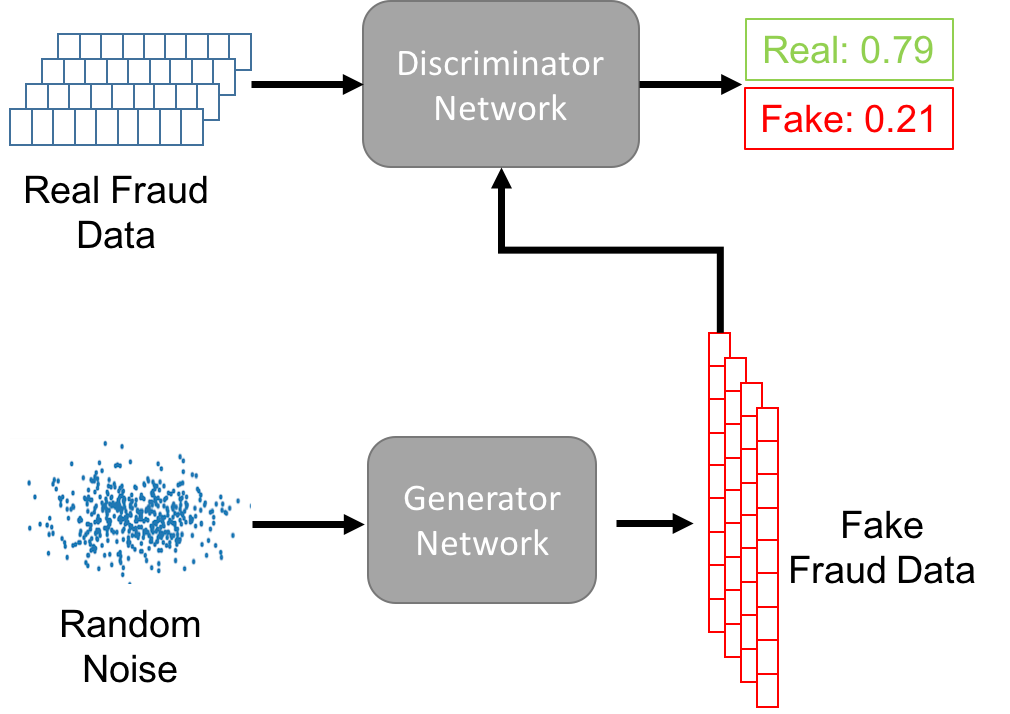
\includegraphics[width=\textwidth]{GAN-Overview}
\caption{Overview of a GAN network}
\end{figure}

Mathematically, we can define the following quantities:

$$X_{x\sim p_\text{data}(x)} = \text{Sample from distribution of real data} $$
$$Z_{z\sim p_\text{z}(x)} = \text{Sample from distribution of generated data} $$
$$G(z) = \text{Generator Network}$$
$$D(x) = \text{Discriminator Network}$$
The process of training for a GAN is like a min-max game between the two networks, and can thus be represented by the following value cost function:
$$\min _ { G } \max _ { D } V ( D ,G )$$
where 
$$V ( D ,G ) = \mathbb { E } _ { x \sim p _ { d a t a } ( x ) } [ \log D ( x ) ] + \mathbb { E } _ { z \sim p _ { z } ( z ) }[ \log ( 1- D ( G ( z ) ) ] $$
The first term in this equation represents the quantity of the real-distributed data passed through the discriminator network. The discriminator tries to maximise this such that $D(x)\rightarrow 1$. The second term represents generated data passed through the discriminator. The generator tries to minimise such that $D(G(z))\rightarrow 1$ (i.e the discriminator is fooled by the generated sample).

The steps for training a GAN can be outlined as followed:
\begin{enumerate}[Step 1:]
  \item 
  \begin{enumerate}
  \item Take a batch of real data and train discriminator to correctly predict them as real
  \item Take a batch of generated data and train discriminator to correctly predict them as fake
\end{enumerate}
  
  \item Freeze the training of the discriminator network
  \item Generate a batch of fake data and use the frozen discriminator to train the generator
  \item Repeat the above for n epochs until neither network makes any further improvments
\end{enumerate}

In summary, we alternate between training of the discriminator to correctly determine real or fake data and training the generator on fooling the discriminator. The reason for freezing the weights of the discriminator while we train the generator is exactly so that we don't alter the weights during this process and the generator can use the current state of the discriminator to become better.

\section{Machine Learning Evalutation Practises}
\subsection{Cross-validation}


\section{Software Engineering}

This section details the project requirements and early design decisions that were made.

\subsection{Requirements}
The main success criteria of the project is outlined as follows:

\begin{enumerate}
   \item Baseline Models
   \begin{itemize}
     \item Compare a handful of supervised learning classifiers, from SciKit-Learn.
     \item Using metrics described in the Evaluation section of the project.
     \item Experiment with resampling techniques. 
     \item Implement appropriate cross-validation.
   \end{itemize}
   \item CNN Models
   \begin{itemize}
     \item Implement CNN version 1 - Single vector input approach.
     \item Implement CNN version 2 - Time series, sliding image window approach.
   \end{itemize}
   \item GAN Models
   \begin{itemize}
     \item Implement GAN version 1 - Dense generator network.
     \item Implement GAN version 2 - Using a CNN model from previous work as the generator network.
     \item Experiment with how GAN is used and how it performs on the data.
   \end{itemize}
\end{enumerate}

 These were all done more or less in order. Some work overlapped, namely work on auxiliary functionality to allow appropriate cross validation or data preparation etc. More details on specifics is outlined in the implementation chapter. 
  
\subsection{Tools and Technologies Used} \label{tools}

Below I describe and justify where necessary the tools and technologies that I used.

\subsubsection{Machine Learning}

I implemented work predominately making use of Keras\footnote{\href{https://keras.io}{https://keras.io}}(with TensorFlow\footnote{\href{https://www.tensorflow.org}{https://www.tensorflow.org}} backend) for CNN and GAN work and SciKit-Learn\footnote{\href{ http://scikit-learn.org/stable/}{ http://scikit-learn.org/stable/}} for baseline models and some general data manipulation/metric functions. 

The reasons for these choices were a mixture of good documentation, popularity \& ease-of-use. Using a TensorFlow backend meant that I could use GPU acceleration if needed. I used Keras as a TensorFlow wrapper, so I could avoid writing models completely from scratch but still giving me the flexibility to develop around models and customise to a large extent. Similarly with SciKit-Learn, which has a lot of helpful utility functions for evaluating models and processing data.

\subsubsection{Version Control and Project Tools}

I hosted my project in a repository on GitHub\footnote{\href{https://github.com/harrygraham/DeepLearning-CreditCardFraud}{https://github.com/harrygraham/DeepLearning-CreditCardFraud}}, used Git for version control, and used virtual environments with pip for project package management and requirements.

I made heavy use of Jupyter Notebooks for writing code in an experimental manner, with immediate execution and feedback. 


\subsubsection{Languages}

My project was entirely written in Python, using the libraries and APIs described previously. This is mainly due to the large ecosystem and documentation surrounding these machine learning libraries in python and also for the ease of use of tools such as Jupyter Notebooks for experimentation.

\subsection{Starting Point}

My project codebase was written from scratch, with the assistance of the tools and libraries mentioned above. Apart from a basic knowledge of supervised learning covered by the part IB Artificial Intelligence course, I had to learn about most of the models and best practises myself, through thorough reading around the topics. 
In terms of technologies, I had little prior experience with SKLearn and Keras/TensorFlow. I had significant experience in Python, however, from a summer internship in industry as well as experience with Git.


\chapter{Implementation}
\section{Models Overview}
\section{Baseline Models}
\section{Convolutional Neural Network Models}
\section{Generative Adversarial Network Models}

\chapter{Evaluation}
\section{Evaluation Methodology}
\subsection{Metrics}
\subsection{Visual Inspections}

\section{Results Overview}

\chapter{Conclusions}

%%%%%%%%%%%%%%%%%%%%%%%%%%%%%%%%%%%%%%%%%%%%%%%%%%%%%%%%%%%%%%%%%%%%%
% the bibliography
\newpage
\addcontentsline{toc}{chapter}{Bibliography}
\bibliographystyle{ieeetr}
\bibliography{references}

%%%%%%%%%%%%%%%%%%%%%%%%%%%%%%%%%%%%%%%%%%%%%%%%%%%%%%%%%%%%%%%%%%%%%

\end{document}





